%===============================================================================
%===============================================================================
%
\clearpage
%
\subsection{Example-0001}
%
%===============================================================================
%
\subsubsection{Mathematical model}
%
We solve the following equation,
%
\begin{align}
    \nabla \cdot \nabla u = 0 & &&\Omega = [0, 2] \times [0, 1] \times [0, 1],
\end{align}
%
with boundary conditions
%
\begin{align}
    u = 0 & &&x = y = z = 0, \\
    u = 0 & &&x = 2, y = z = 1.
\end{align}
%
No material parameters to specify.
%
%===============================================================================
%
\subsubsection{Computational model}
%
\begin{itemize}
    \item{Length, width, height}
    \item{Direct/iterative solver}
    \item{Generated/user mesh}
    \item{Number of elements}
    \item{Interpolation order}
    \item{Number of solver steps (time steps, load steps)}
\end{itemize}
%
%===============================================================================
%
\subsubsection{Results}
%
\begin{figure}[h!]
    \centering 
    \includegraphics[width=\columnwidth]{examples/example-0001/doc/figures/analytical_solution.eps} 
    \caption{Results, analytical solution.}
    \label{example-0001-analytical-solution-fig}
\end{figure}
%
\begin{figure}[h!]
    \centering 
    \includegraphics[width=\columnwidth]{examples/example-0001/doc/figures/abaqus_reference.eps} 
    \caption{Results, Abaqus reference.}
    \label{example-0001-abaqus-reference-fig}
\end{figure}
%
\begin{figure}[h!]
    \centering 
    \includegraphics[width=\columnwidth]{examples/example-0001/doc/figures/iron_reference.eps} 
    \caption{Results, iron reference.}
    \label{example-0001-iron-reference-fig}
\end{figure}
%
\begin{figure}[h!]
    \centering 
    \includegraphics[width=\columnwidth]{examples/example-0001/doc/figures/current_run.eps} 
    \caption{Results, current run.}
    \label{example-0001-current-run-fig}
\end{figure}
%
%===============================================================================
%
\subsubsection{Validation}
%
CHeart rev.\ 6292, Abaqus 2017, analytical reference solution, whatever...
%
%===============================================================================
%===============================================================================
